% Fig. A.3 — regenerated by scripts/09_export_paper_figures.py
% from results/tables/b9_same_ckpt_destruction.csv (fold-0 node-drop).
\begin{figure}[htbp]
\centering
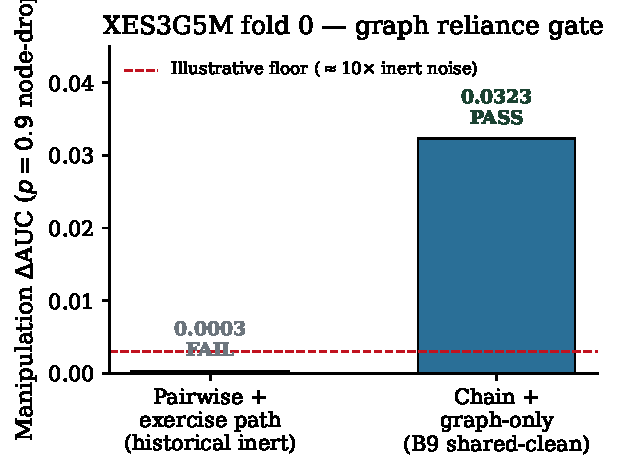
\includegraphics[width=0.92\columnwidth]{figures/fig_manipulation_sweep.pdf}
\caption{Manipulation-check $\Delta$AUC on XES3G5M fold~0 under $p{=}0.9$
node-drop. The right bar is the B9 shared-clean evaluator
($\Delta$AUC$=0.0323$; Table~\ref{tab:manipulation}). The left bar is a
historical graph-inert path ($\Delta$AUC$\approx 0.0003$) and is
\emph{not} that evaluator. The dashed line at $0.003$ is an
\emph{illustrative} floor ($\approx$10$\times$ the graph-inert noise),
not a formal statistical cutoff from \cite{daominh2026p0}.}
\label{fig:manipulation-sweep}
\end{figure}
